%latex.default(figure1)%
\documentclass{article}
\usepackage[pdftex]{graphicx}
\begin{document}
\begin{figure}
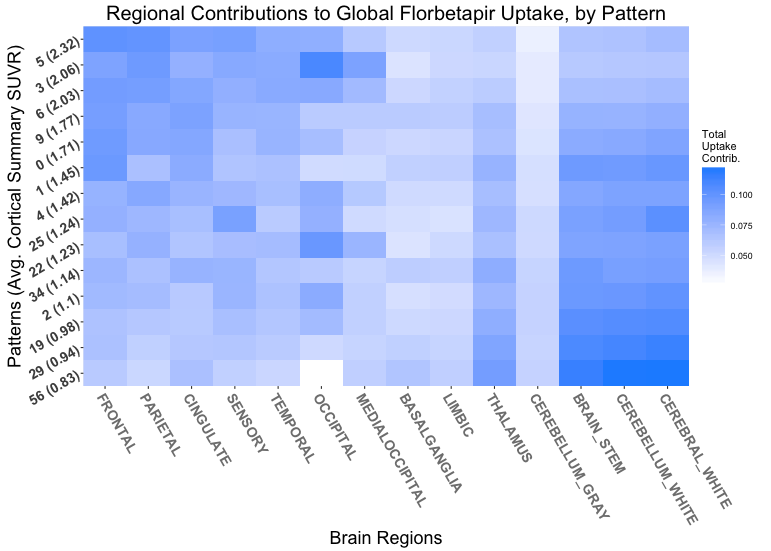
\includegraphics[width=125mm]{/usr/local/jagust/lobe_contributions.png}
\caption{The columns map to brain regions, while each row represents an uptake pattern, sorted by the average cortical summary SUVR of its members. Each uptake pattern is broken down by uptake contribution per region, i.e. regional SUVR divided by summed SUVR across all brain regions, and thus the values in each row sum to 1. Uptake contributions range from 0.03 to 0.12, presented on a white (low) to blue (high) spectrum.}
\end{figure}

\begin{figure}
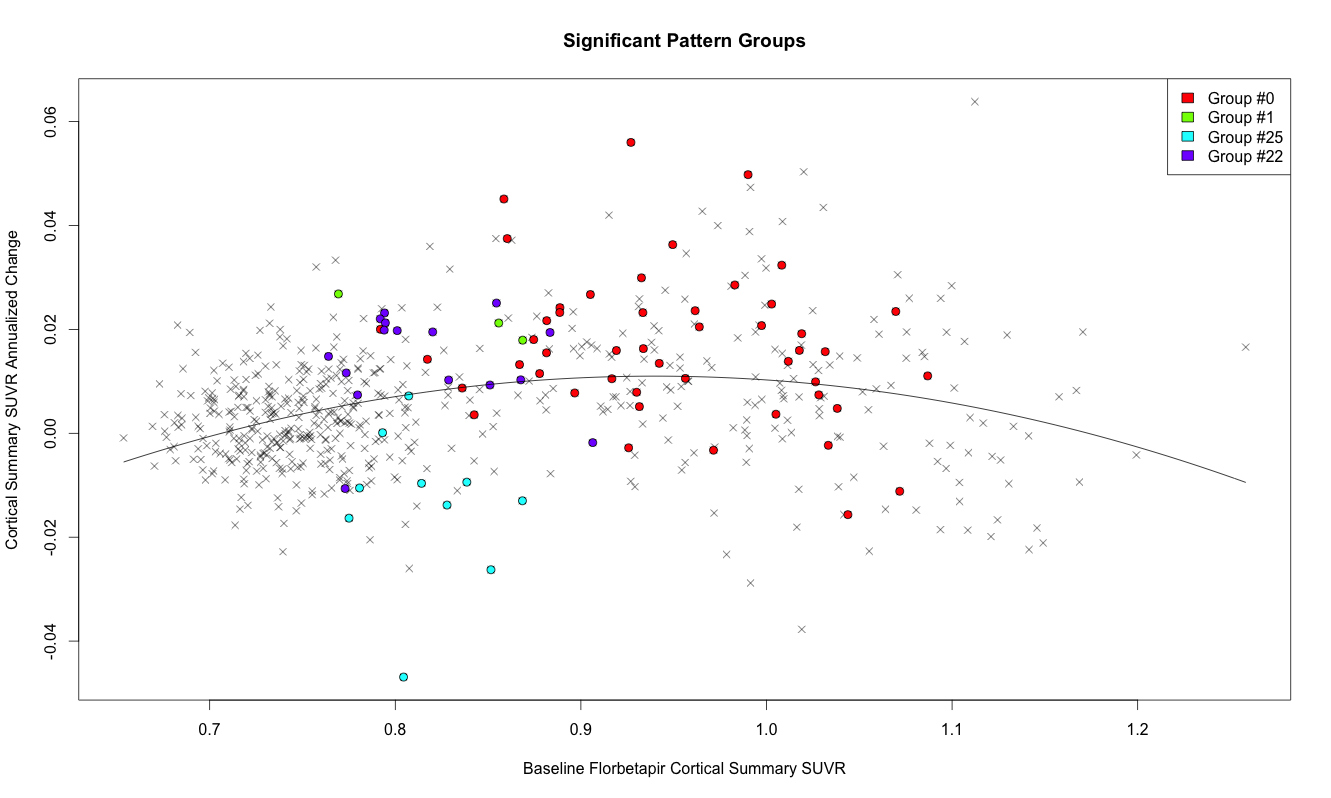
\includegraphics[width=125mm]{/usr/local/jagust/fitplot_sigpatterns.png}
\caption{Each point represents the pre-existing relationship between baseline florbetapir cortical summary SUVR and subsequent annualized change in SUVR, for 368 CN and 554 MCI ADNI subjects. The black line represents predicted annual change by baseline SUVR. The colored points represent members of the pattern groups which exhibit significant effects on annualized change, despite correcting for non-pattern factors including baseline SUVR, age, sex, education, and Apoe4 status.}
\end{figure}


\end{document}